\section{Implementation}\label{sec:implementation}
\subsection{Virtual Plug-and-Play Network}
\subsubsection{Design}
The goal with the first implementation was to test the capabilities of VPPN.
This included basic infrastructure such as a Lookup Service, a CAN bus
gateway, an application (a consumer of data) and a service provider. Figure
\ref{fig:vppn-overview} shows the basic components needed and how they are
interconnected in suggested minimal implementation.

\begin{figure}[h]
    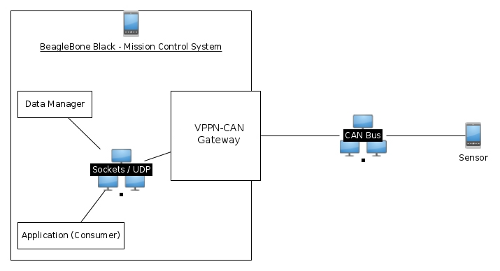
\includegraphics[width=0.5\textwidth]{./figure/vppn-overview.png}
    \caption{Overview of the minimal VPPN design with CAN bus Gateway.}
    \label{fig:vppn-overview}
\end{figure}

Each component's responsibility is described in the following list and an
example connecting all components together is presented after that.
\begin{itemize}
    \item {\em Lookup Service (LS)} keeps track of all connected components
        respective interfaces (available and required data).
    \item {\em Application (consumer)} uses data supplied by the service
        provider.
    \item {\em Service Provider} could be a sensor of some kind that
        applications can subsribe to for reguarly updates of the sensor value.
    \item {\em VPPN-CAN Gateway} routes traffic from the local subnet in the
        processing unit to the CAN bus local subnet.
\end{itemize}

In a fully operational VPPN network adress resolution and initial
configuration is partly done by other components not used in this minimal
design, for the minimal implementation hardcoded settings were planned instead.

After initial configuration each component sends information to the
Lookup Service when requested in the format of "Extensible Transducer Electronic Data Sheets"
(xTEDS) which is a XML file with a predefined structure. This file includes
respective components interfaces and must be created when the component is
constructed (it should be stored together with the component it describes).

The Lookup Service then goes through all xTEDS to find out which components
require information from other components. The Lookup Service in the minimal
implementation would find that the "Application" requires sensor information of
the same type the "Service Provider" supply. The Lookup Service would then report
back to the Application with information that the Application should contact
the Service Provider. The Application would then ask for required data or
subscribe to the Service Provider's sensor information in a peer to peer manner.

Whenever the Service Provider on the CAN bus subnet communicates with another
component outside of the CAN bus subnet the VPPN-CAN Gateway routes the traffic.
To be able to do this routing, the VPPN-CAN Gateway is also
responsible for the adress resolution in the boot up phase for the CAN bus
subnet.

\subsubsection{VPPN and CAN bus}\label{subsubsec:vppn_can_bus}
In the minimal design the VPPN-CAN Gateway component runs on the same
processing unit as the Mission Control System and connects with other
components on that local subnet through UDP/IP through the loopback interface.

In a VPPN network each component, both hardware and software, must have a unique
logical address. When starting the system the responsiblity of the VPPN-CAN Gateway is to
enumerate the CAN bus for all connected components and assign a local subnet address to
each one. This contradicts the behaviour of the CAN bus which is message based
and not address based. As per request from the customer the project went
forward with the minimal implementation design without putting any attention to
the contradiction.

The main issue to solve is the assignment of addresses. In IP networks and VPPN Local
Subnets a common address is used to make the network manager aware of the newly
connected component. For IP networks newly connected network devices send a
broadcast message to all other devices on the same local network with it's own
address as 0.0.0.0 (IPv4). The DHCP server then replies with a response that
includes a new IP address the device can use. In the SPA Local Subnet
Adaptation Draft newly started processes sends a message to the loopback
interface at port 3500 requesting an address. Together with the request for a
new address a unique identifier is included in the message (e.g. MAC Address
for IPv4 networks).

Applying the same behaviour to the CAN bus would cause the CAN bus to
malfunction due to collision errors when multiple CAN hosts transmit the same
message ID but with different payloads (including the unique identifier).
This is related to the bootstraping problem others have tried to solve with
"IP over CAN" \cite{web:draft-ip_over_can, web:porting_ip_can}.

For the minimal implementation the project went forward with inspiration from
Ditze et. al \cite{web:porting_ip_can} where the 29 bits message ID from the
CAN bus 2.0B specification is divided into different subparts. It starts with a 10
bits prioritisation band, 3 bits message type field, 8 bits sender address and
the last 8 bits represent destination address. This can be seen in table
\ref{table:mapping_message_id_to_ip}.

\begin{table}
\centering
    \caption{Mapping of message ID for address based communication over CAN
    Bus.}
    \begin{tabular}{|c|c|c|c|} \hline
    \label{table:mapping_message_id_to_ip}
    Prioritisation & Msg & Sender Address & Dest. Address  \\ \hline
            10 bits & 3 bits & 8 bits & 8 bits \\ \hline
    \end{tabular}
\end{table}

To eliminate the problem with collisions on the CAN bus unique component
identifiers must be used within the message id. One solution explored was to
define a message type as "DHCP" request and use both the sender and destination
address as a 16 bits unique data field. 16 bits is not enough for MAC addresses
used in IPv4 devices (48 bits), unique identifiers in IPv6 devices (64 bits)
nor the 128 bits CUUID used within VPPN. At this point no further work took
place regarding this topic.

\subsubsection{VPPN and Ada}
During the initial implementation phase focus was put on Ada functionality and
getting the communication between software components working. UDP/IP and TCP/IP
were tested and it was clear early on that UDP/IP wouldn't work very well so
the project continued with testing TCP/IP together with Ada Tasks more
thoroughly. It was during a meeting with the customer at this point in the
project the customer made clear that sockets were a no-go. TCP/IP communication
was dropped in favour of "Protected Objects" from the Ada language for
inter-process communication.

At this point it was decided to drop VPPN from the project, prioritising other
requirements from the customer.

% \begin{figure}[h]
%     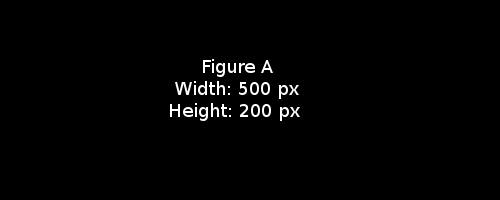
\includegraphics[width=0.5\textwidth]{./figure/figureA.png}
%     \caption{Figure A}
% \end{figure}
%
% \subsubsection{Subsubsection1}
% Test of two columns figure. It should be shown at the top of a page.
% \begin{figure*}[t]
%     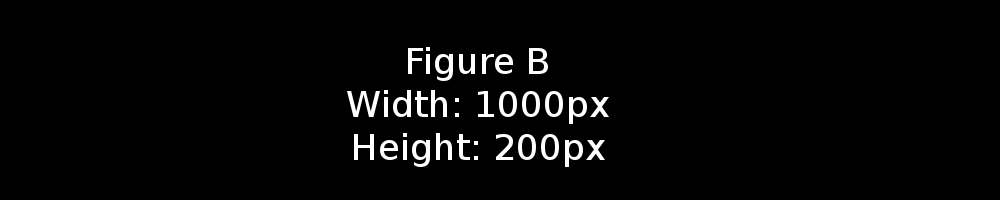
\includegraphics[width=1.0\textwidth]{./figure/figureB.png}
%     \caption{Figure B}
% \end{figure*}
